% vim: set fenc=utf-8 ft=latex encoding=utf-8
% -*- mode: latex; coding: UTF-8; -*-

\newif\ifdraft
\drafttrue

\ifdraft
	\documentclass[conference, draftclsnofoot]{IEEEtran}
	\def\baselinestretch{1}
	\setlength{\marginparwidth}{2cm}
\else
        \documentclass[conference]{IEEEtran}
	\def\baselinestretch{1}
	\setlength{\marginparwidth}{2cm}

	% \documentclass[conferece, final]{IEEEtran}
\fi

\usepackage[T1]{fontenc}
\usepackage[utf8]{inputenc}

\newcommand{\TheTitle}{Visualizing Release Information of Linux}
\newcommand{\TheAuthors}{Evan Wilde}
\newcommand{\TheEmails}{etcwilde@uvic.ca}
\newcommand{\TheSubject}{Digesting large amounts of commit data}
\newcommand{\TheKeywords}{Linux, git, data structures, tree data structures}

\synctex=1

\usepackage[hyphens]{url}
\urlstyle{same}

\ifdraft
	\usepackage[unicode=true,bookmarks=false,breaklinks=false,
		pdfborder={0 0 0},backref=none,colorlinks=true]{hyperref}

\else
	\usepackage[unicode=true,bookmarks=false,breaklinks=false,
		pdfborder={0 0 0},backref=none,colorlinks=false]{hyperref}
\fi

\usepackage[nospace]{cite}

% Table Support
\usepackage{dcolumn}
\usepackage{longtable}

\usepackage{balance}
\usepackage{placeins}
\usepackage{multirow}

% Extra support
\usepackage{xspace}
\usepackage{caption}
\usepackage[nospace]{cite}

% Fix any bad-hyphenations here
\hyphenation{}

% \ifdraft
%     \usepackage[colorinlistoftodos]{todonotes}
%     \newcommand{\evan}[1]{{\color{blue}\emph{Evan Says: #1}}\xspace}
%     \newcommand{\evantodo}[1]{{\color{blue}\emph{Evan Todo: #1}}\xspace}
%     \newcommand{\dmg}[1]{{\color{blue}\emph{dmg Says: #1}}\xspace}
%     \newcommand{\dmgtodo}[1]{{\color{blue}\emph{dmg Todo: #1}}\xspace}
% \else
%     \usepackage[disable]{todonotes}
%     \newcommand{\evan}[1]{}
%     \newcommand{\evantodo}[1]{}
%     \newcommand{\dmg}[1]{}
%     \newcommand{\dmgtodo}[1]{}
% \fi
    \usepackage[colorinlistoftodos]{todonotes}

\newcommand{\tool}{{\emph Linvis}\xspace}


    \newcommand{\evan}[1]{{\color{blue}\emph{Evan Says: #1}}\xspace}
    \newcommand{\evantodo}[1]{{\color{blue}\emph{Evan Todo: #1}}\xspace}
    \newcommand{\dmg}[1]{{\color{blue}\emph{dmg Says: #1}}\xspace}
    \newcommand{\dmgtodo}[1]{{\color{blue}\emph{dmg Todo: #1}}\xspace}


%%% Local Variables:
%%% mode: plain-tex
%%% TeX-master: t
%%% End:


\begin{document}

\title{\TheTitle}
\author{
\IEEEauthorblockA{\TheAuthors}
\IEEEauthorblockN{Department of Computer Science,
                    University of Victoria, Canada.}
\IEEEauthorblockA{Email: \TheEmails}
}
\maketitle
\begin{abstract}
	With an average of over 900 top-level merges into the Linux kernel per
	release, some containing thousands of commits, many containing hundreds
	of commits, maintenance of older versions of the kernel becomes nearly
	impossible. For security, performance, and changing hardware needs,
	maintainers must understand the changes made to current versions of the
	kernel, and understand how these changes fit into older version in
        order to make the necessary merges and modifications to the older
        versions. Current tools provide information about repositories through
        the directed acyclic graph (DAG) which is helpful for smaller projects,
        but with the scale and number of branches in the kernel, the DAG
        becomes overwhelming very quickly.

	In this paper, we present a tool that uses the dataset collected by
	German et al. to build a tool that uses a tree-based model instead of
        the DAG. This tool is designed to cater to the needs of users looking
        for a top-down approach, or a bottom-up approach to navigating the
        commit information of the kernel.
\end{abstract}

\begin{IEEEkeywords}
\TheKeywords
\end{IEEEkeywords}

\section{Introduction}

Maintainers of older version of the Linux kernel must sift through thousands of
commits with tools that are unable to filter and effectively visualize projects
that are of the scale of the kernel. Tools like Gitk provide users with the
full view of the DAG, showing all merges and commits. For smaller projects,
this information is useful for showing the relation between various branches.
The DAG becomes a tangled mess (\ref{fig:gitk}) of commits, merges, and the
links between them with large modular projects, like the Linux kernel. This
makes it difficult to derive an explanation of the changes made. In other
cases, the kernel is simply too large for the system to generate a
visualization for. Github provides a DAG view for most projects, but is unable
to display the visualization for projects as large as the Linux kernel.

\begin{figure}
	\centering
	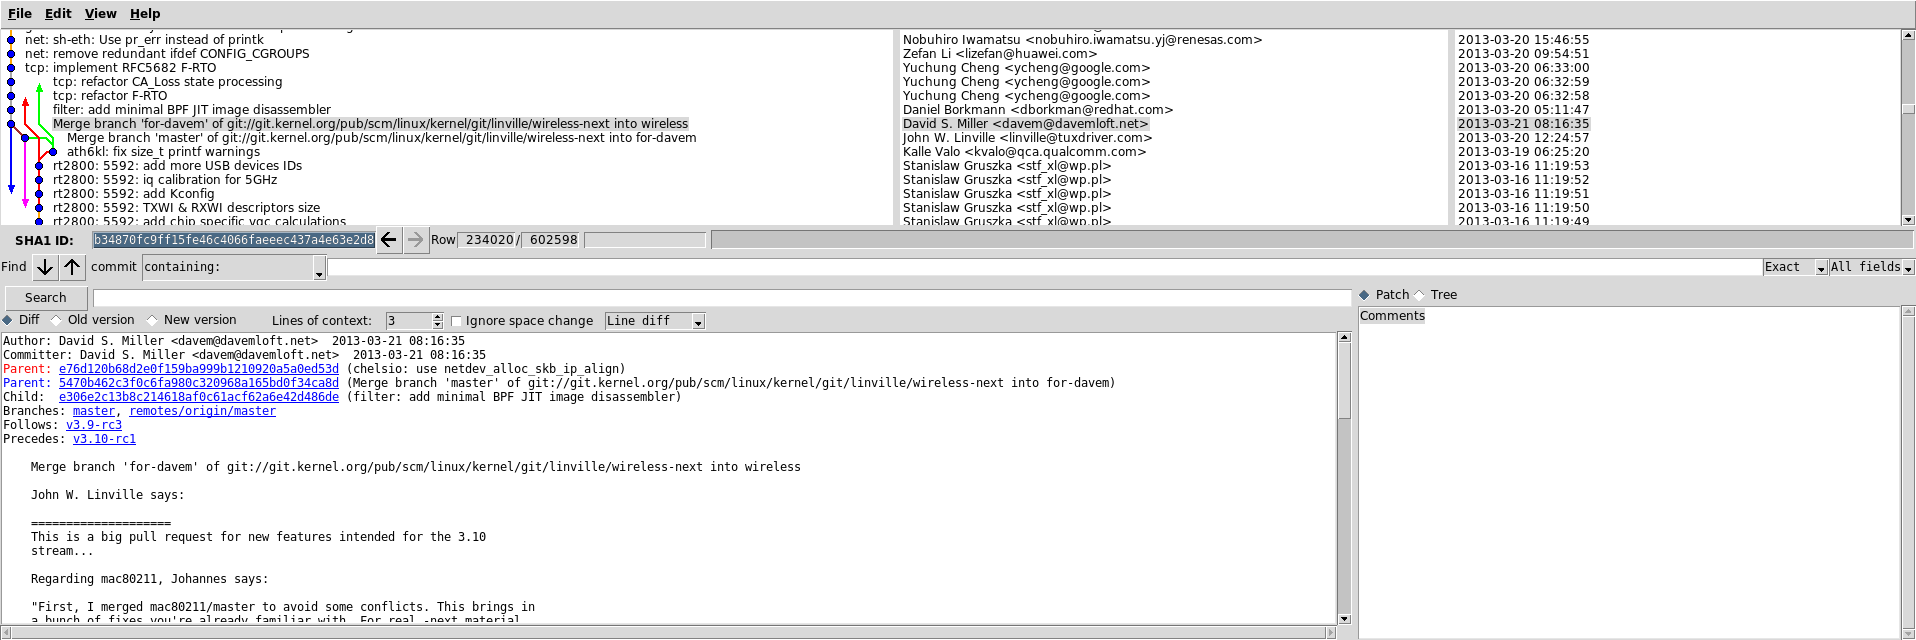
\includegraphics[width=0.47\textwidth]{figures/gitk.png}
	\caption{DAG view in Gitk}
	\label{fig:gitk}
\end{figure}

Git log, Gitk, and other similar tools only store the authored date of a
commit. A commit may be merged into the project at any time, regardless of when
the commit was authored, making date-range queries meaningless. Performing a
date-range query using other tools over the span of a release will contain
results that are for previous versions of the kernel, and may not contain all
of the results for that kernel if patches were merged after the release date.

German et al. recorded the metadata of every commit and merge in the Linux git
repository starting in 2011 \cite{German}, including chronological data that is
not stored by git. We are able to use this information to generate sets of
trees instead of a DAG. The root of each tree is the top-level merge performed
by Linus, which merges branches or sets of commits into the kernel.

In this paper, we present the design decisions behind a web-based
tool\footnote{\url{http://li.turingmachine.org}} built around a tree-based
model instead of the DAG.  We demonstrate the advantages of this model over the
DAG two main use-cases.  Our tool provides information about the location of a
given commit in the respective merge tree, the files edited, the modules
edited, and the commit message in a given commit or merge.  The tool allows
users to apply various filters, including the release, a keyword or phrase from
the log preview, the name of the author, or the commit id. The user can request
all the top-level merges containing a commit or merge that matches the query,
or all commits and merges that match the query.

Our core model provides advantages to the DAG model used by other tools.
Breaking the commits and merges by merge tree removes the commits and merges of
other components of the kernel from the visualization, providing a clearer
picture of what is happening in a given merge. This model provides additional
support to edited file information. Furthermore, we are able to understand the
changes being made in the order they are brought into the kernel.

All top-level merges to a given version of the kernel are merged between the
start and release date. Our tree construction allows us to use the top-level
merges to find all merges and commits that have an effect on a given version of
the kernel. The model allows us to better provide mechanisms for performing
date-range queries, providing access to all commits that have an effect on a
given release, even if the commit comes before the start date, or after the
release date.

\section{Related Work}

To our knowledge, no repository visualization systems using a tree-based model
are being used. This may be due to the fact that more information than what
is stored by the normal tools is required to create the trees, so servers must
sit and watch as the repository changes over time. Many of the visualization
tools are designed for a general-purpose approach, where any repository is
directly usable, without additional information. Polling for this additional
information makes the application specific to a single repository, or project.

\subsection{Gitk}
Gitk, Gitg, and other similar git repository visualizing tools use the DAG as
the central organization. For smaller projects, this model is sufficient for
providing meaningful information, but in larger projects like the Linux kernel,
the branches become too tangled and too deep to derive any meaning from the
DAG. The DAG model allows users to go to the next commit in the chain, go to
the previous commit in the chain, or jump to the parent merge. This suggest
that Gitk and similar tools are designed for users working with a bottom-to-top
approach. With this model, it is difficult for users to see what other commits
are involved with a given merge. Gitk only provides file information on
commits, as it is unable to quickly find all files edited by a merge. It is up
to the user to remember what files were edited in each of the commits involved
in a given merge. In some of the larger merges, some containing over 1500
edited files, this task become nearly impossible.
% cid: 73287a43cc79ca06629a88d1a199cd283f42456a, 1800 commits, 1500 files
Other DAG visualization systems, like the GitHub viewer (\ref{fig:gitfail}),
are unable to provide a visualization for projects that are as large as the
kernel.

\begin{figure}[h!]
	\centering
	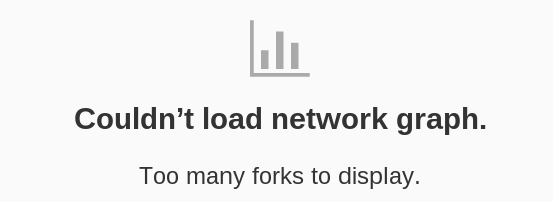
\includegraphics[width=0.45\textwidth]{figures/github_viewer.png}
	\caption{Github Failure Message}
	\label{fig:gitfail}
\end{figure}

%% Check for papers if they exist
%% This tool isn't specifically designed for showing Linux

\subsection{Treemap visualizer}
University of Maryland presented a treemap visualization
tool\footnote{\url{https://www.cs.umd.edu/hcil/millionvis/Treemap_Visualization_of_the_Linux_Kernel_2_5_33.html}},
pictured in figure \ref{fig:treemap}, for
displaying all the file structure of a given version. Treemaps are good for
displaying the topology of shallow, wide trees, making it a good candidate for
displaying file systems. Treemaps are limited in what information can be
displayed. The information within the treemap does not provide clear insight on
what changes were made to the files in the given release. The treemap
visualization only provides information on where the file is located within the
filesystem. File systems and the merge tree of the kernel share many
similarities, in both cases, the representative trees are wide and shallow,
suggesting that a treemap could potentially work to visualize the commit and
merge structure of the kernel.

The treemap is unable to take into account multiple merges at the same level
with the same name. There is an additional dimension, in that the commits and
merges are ordered in time. The treemap design is unable to show the ordering
of the merges and commits.

The treemap design is also designed for working with data of differing types.
In the filesystem, there are many kinds of files.  There are text files,
scripts, images, binary files, and other types. These can be given colours
making differences stand out. There is no obvious way to assign meaningful
types to the commits such that all the commits within a given merge do not all
have the same colour.

Finally, the treemap does not provide any additional information about the
contents of each cell, only that the cell exists. The user is unable to see
their current position within the map, or if we assume that their current
position is the larges surrounding box, they can no-longer see how their
current position interacts with the rest of the system.
%% https://www.cs.umd.edu/hcil/millionvis/Treemap_Visualization_of_the_Linux_Kernel_2_5_33.html
%% Find paper for this maybe?

\begin{figure}[h]
	\centering
	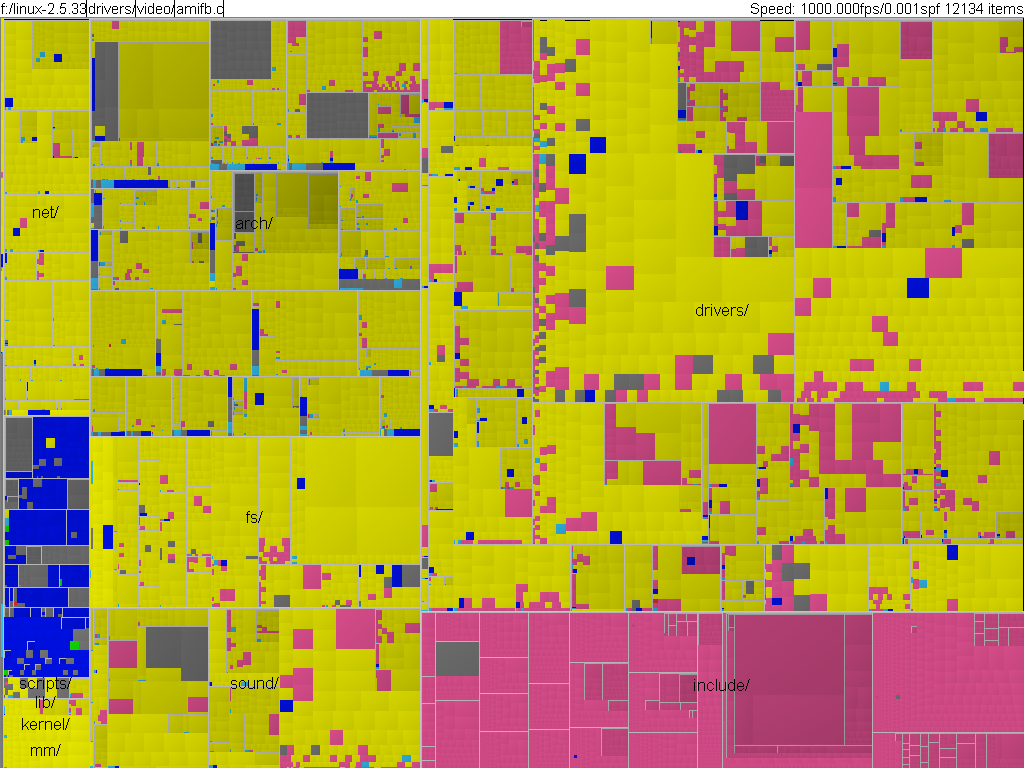
\includegraphics[width=0.47\textwidth]{figures/kernel-files.png}
	\caption{Treemap of Linux 2.5.33 file structure}
	\label{fig:treemap}
\end{figure}

\subsection{List viewer}
Moghaddam designed a web-based visualization
tool\footnote{\url{http://web.uvic.ca/~arasbm/gitVisualizations/linuxRGraph.html}}
displaying the chain of merges into the kernel. There is no information on what
commits are within a given merge, or what files were edited. The visualization
tool provides information about who authored the commit and when it was
authored. We can see the visualization tool in figure \ref{fig:listviewer}
displaying a part of the kernel commit information, from commit ``26b23ac''
according to the tool.

%% http://web.uvic.ca/~arasbm/gitVisualizations/linuxRGraph.html
%% Find paper for this maybe?

\begin{figure}[h]
	\centering
	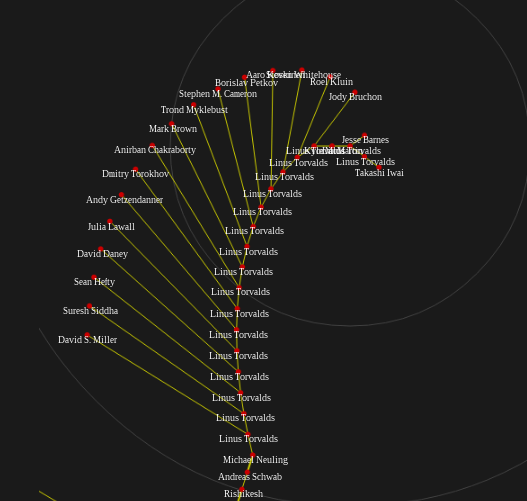
\includegraphics[width=0.47\textwidth]{figures/gitvis.png}
	\caption{List Viewer}
	\label{fig:listviewer}
\end{figure}


\section{Design}

The goal is to build a tool that make navigation of the kernel commit
information simpler, while providing an explanation of the changes occurring at
each commit and merge. Part of making the information usable is to narrow the
results down into only the information that is relevant to what the user is
looking for. We designed the tool with two use-cases in mind, though a user may
switch roles many times as they work.

\textit{Use-case 1: top-to-bottom approach}\\
These are users that are maintaining a section of the kernel and would like to
pick a merge from the future merges and merge it directly into their current
repository. This is useful for minimizing required implementation on the side
of the maintainer. We must provide them with methods of navigating from a more
general set of merges toward a specific set of merges and commits.

\textit{Use-case 2: bottom-to-top approach}\\
These are users that know what merge or commit they are working with and would
like to see what else is happening around their current commit. This is useful
to see how changes to a given file will break other changes made by other
commits. This is primarily for maintainers that have to perform some
implementation work in order to correctly merge the patches from the future.
These users may also know what module(s) they are dealing with, and are looking
for modules that are relevant to the area they are working on. We must provide
them methods of navigating from a specific commit to a more general merge,
allowing them to see a bigger picture.

\subsection{Core Model}
Each top-level merge into the kernel is the root-node to a tree. Each merge
may contain zero or more children of other merges or commits. Commits have no
children, and therefore are always leaf nodes, but commits contain information
about what files are edited and how many lines are edited, along with what
modules are involved in a merge.

\subsection{Command-line Shell}

Our initial intuition was to work with the commits and merges as trees, like in
a file structure. There are many similarities in the structure of a file system
and the structure of the commit information within the kernel. The primary
similarity is that they are both trees, and both trees are generally fairly
shallow and very wide. File systems have been around for quite some time, and
there are many tools for visualizing and working withe the file structure. The
first tool was the command-line. We built a small command-line shell
(\ref{fig:shell}) that allowed navigation through the commit and merges instead
of files and directory. The shell design permitted a user to move through the
merges like they would through directories. They could use the cat command to
see the preview of the log, or the more command to see the preview and what
files were edited in the commit and how many lines were added and removed from
each file.

\begin{figure}[h]
	\centering
	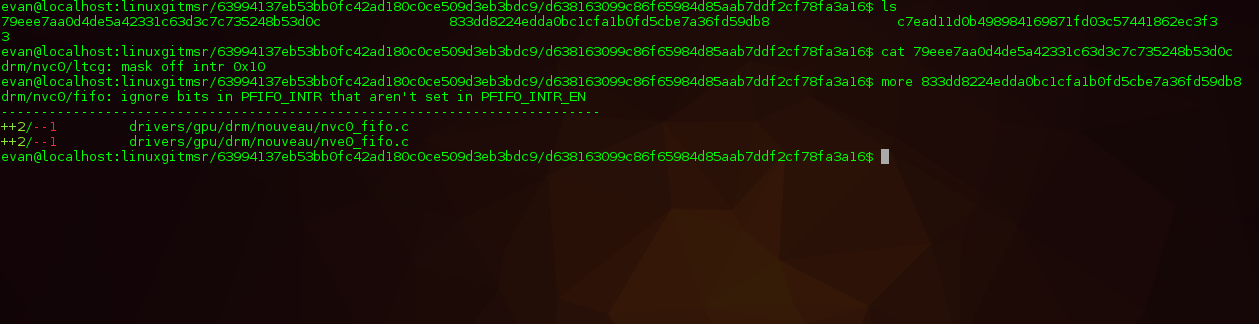
\includegraphics[width=0.47\textwidth]{figures/shell.png}
	\caption{Shell Design}
	\label{fig:shell}
\end{figure}

There are two issues with this design. One issue with this design is that a
user will always move from the top-down without any additional filtering. This
only serves one of our use-cases. The second issue being that it presents the
user with the commit hashes, providing no explanation of what the commit or
merge may contain.

\subsection{Web-based Tool}

There are multiple reasons for building the system into a web-based tool.
Putting the tool on the web enables users to use the system without having to
install any software, making the system more accessible and platform
independent.A web-based tool can utilize more interactive means of navigation,
and provide a better explanation of what each commit or merge may contain than
the command-line variant.

Our implementation of the web-based tool provides many mechanisms to enable
users to better navigate and understand changes in the kernel. These mechanisms
include searching, commit messages, files edited, modules edited, and two types
of tree viewers.

\begin{figure}[h]
	\centering
	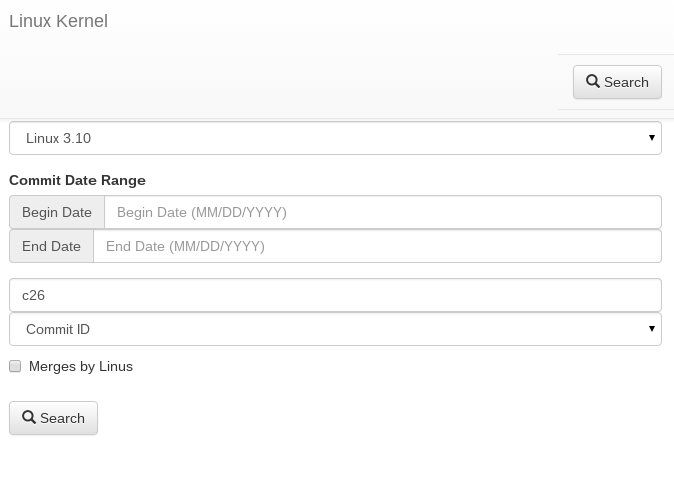
\includegraphics[width=0.47\textwidth]{figures/search.png}
	\caption{Search View}
	\label{fig:search}
\end{figure}

Searching allows a user to filter our commits and merges that are irrelevant.
The search mechanism breaks down the results by release version. A user can
further narrow down the search range using the commit date range. This commit
date refers to the date of the creation of the top-level merge. Commits and
merges that are returned may have a commit date beyond the given range if they
were merged to a top-level merge within the date range. A user may then provide
a search text, filtering on the author name, the commit id, or keyword from the
log. Any part of the author name may show up in the results, including
searching by email address. The commit ID must be specified from the first
character to the last character. For example, the commit
`c267548755a184ef97301071300c1739a564e135' is returned when the user searches
for a commit id of `c26' in the 3.10 Linux kernel.

\begin{figure}[h]
	\centering
	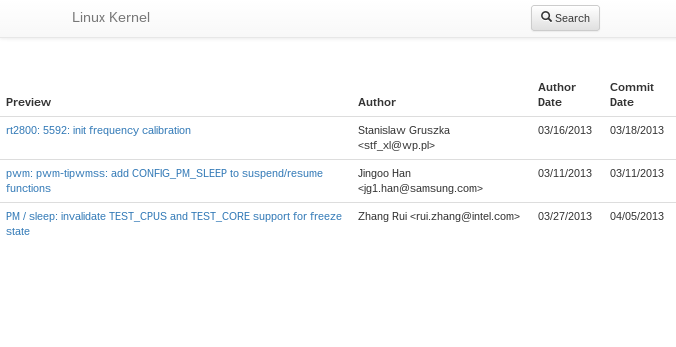
\includegraphics[width=0.47\textwidth]{figures/search_results.png}
	\caption{Search Results}
	\label{fig:results}
\end{figure}

In the search results , the user is presented with the one-line log message
preview, the author's name and email, the date the commit was authored, and the
date the commit was committed. \evantodo{a better definition for commit date}
The commit date and author date will usually be the same, however, if the
commit has been rebased, the commit date will be different than the authored
date, and will always be after the authored date. The first and third entries
in figure \ref{fig:results} have been rebased in the past. \evan{We are unable
to show the rebases.}

\begin{figure}[h]
	\centering
	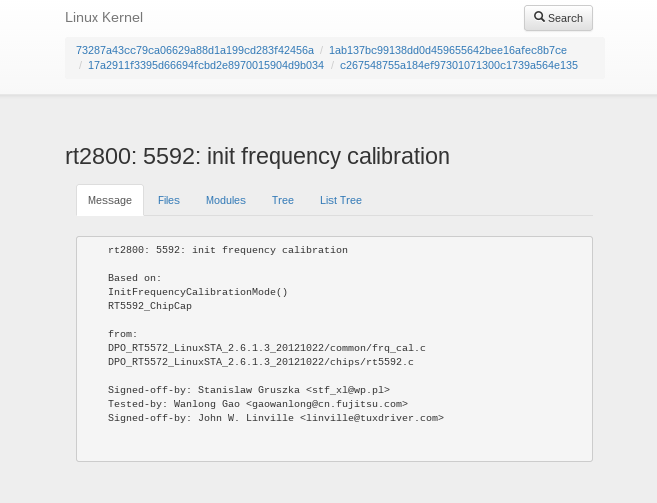
\includegraphics[width=0.47\textwidth]{figures/message_view.png}
	\caption{Commit Message}
	\label{fig:message}
\end{figure}

The first view displays the full commit log. From this, a user is able to see
hat they would see had they searched for the commit using git log. This doesn't
provide additional information to the other tools, but helps to complete the
functionality of the tool. This information provides a user with the
information about the content of the commit and who has looked over the commit
to ensure that it is good quality. The message for merges may also contain the
information about the commits that are being merged into a given merge. The
information within these messages is highly variable, and is completely
dependent on the author's style. As the user moves toward the top-level merge,
the quality of these messages generally improve.

\begin{figure}[h]
	\centering
	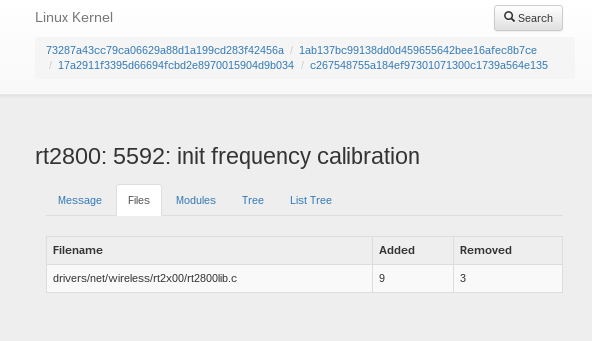
\includegraphics[width=0.47\textwidth]{figures/file_view.png}
	\caption{Commit Files}
	\label{fig:files}
\end{figure}

The second tab is the files tab. This tab provides information on what files
have been edited, how many lines were added, and how many lines were removed in
a given commit. This functionality is similar to the other tools available. Our
tree-based design model allows us to extend this functionality to merges, which
the other tools are unable to show. When a file is edited multiple times from
different commits within a merge, we simply add the added and removed lines to
the values already stored. \evan{At this time, we don't have a mechanism to
process the diff information to determine which lines were changed, and in what
order.}

\begin{figure}[h]
	\centering
	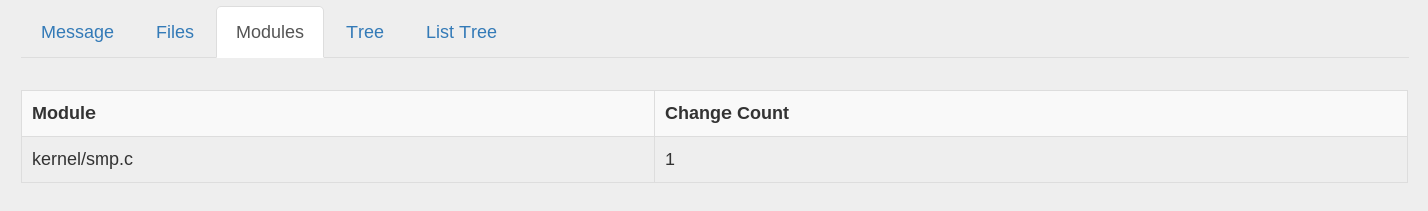
\includegraphics[width=0.47\textwidth]{figures/modules.png}
	\caption{Commit Modules}
	\label{fig:modules}
\end{figure}

The modules tab shows the modules that are contained within the commit. Modules
are not natively recognized by git, and are not going to be present in all
repositories. In the Linux repository, authors put the module they are working
on in the one-line preview of the log-message.  We heuristically extract the
module by taking all text in the log preview until the first colon. Modules are
logical partitions of the information in the kernel. Depending on where the
author was working, modules can be general, such as ``bluetooth'' and
``wireless'', or can be quite specific for individual hardware, such as
``ath9k\_hw'' and ``wl1251''. Like files, we are able to show what modules are
edited in merges and in commits. The image in figure \ref{fig:modules} shows
the modules for a commit. A commit will only ever have one module that it is
associated with.

\begin{figure}[h]
	\centering
	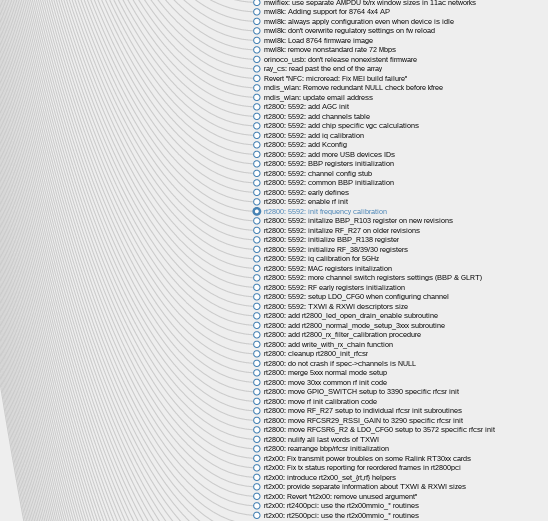
\includegraphics[width=0.47\textwidth]{figures/tree_view.png}
	\caption{Commit Tree View}
	\label{fig:tree}
\end{figure}

The third tab shows the tree view (\ref{fig:tree}). The tree view is what makes
this tool unique to the other tools. It provides a full view of the entire
merge tree. It originally centres at the current commit or merge, but allows a
user to inspect the other commits and merges surrounding it. A user may then
navigate to any of the commits by simply double-clicking on it.

\begin{figure}[h]
	\centering
	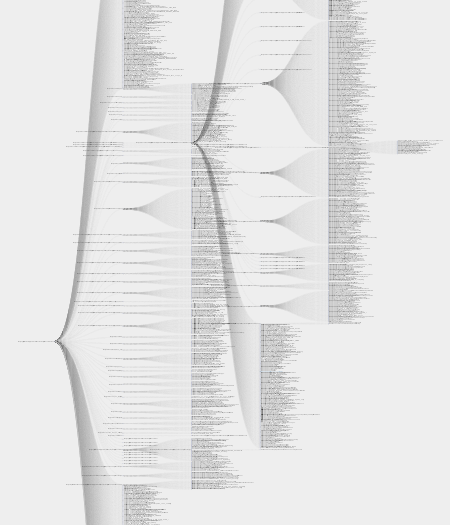
\includegraphics[width=0.47\textwidth]{figures/tree_zoom.png}
	\caption{Tree zoomed out}
	\label{fig:zoomed_tree}
\end{figure}

Some of the merge trees are very large (\ref{fig:zoomed_tree}), containing
thousands of commits and merges. Clicking on subtrees will cause them to
minimize, only showing parts of the tree that are of interest to the user.
Furthermore, the user can zoom the tree by scrolling the mouse wheel to see
more of the topology of the tree, or to see the details of a given part of the
tree.

The last tab contains another type of tree view. This tree is in the form of
nested lists, and is designed to more closely model the tree hierarchy view of
file browsers. This tree only contains the commits and merges that are within
the subtrees of the current merge. A commit will never have any items in this
tab, as it is a leaf node, so it cannot contain subtrees. To accompany the
tree, we include breadcrumbs at the top. The last item in the breadcrumb list
is the current commit, the next item is the parent of the current commit, and
the first item is the top-level merge into the kernel.



\section{Implementation Details}

We built a we-based tool to provide information about the kernel.
We chose to use Nginx as the main web server, postgresql as the dbms, and Flask
as the framework for generating the dynamic content.

Nginx is a high-performance, scalable HTTP and mail server. Started in 2002,
the project is much younger than the Apache project, and designed with massive
scalability and multi-processing in mind. Instead of using request-driven
threading, Nginx uses an event-driven architecture, making it more scalable,
proving itself as being the web server behind Netflix, Hulu, GitHub, Tumblr,
and many other popular sites.

Postgresql is our dbms of choice, providing fast and reliable results. There
are multiple reasons behind choosing postgresql over another dbms. The main
reason being that the dataset provided from \evantodo{paper} was generated from
a postgresql database, allowing us to import the data directly without any
further conversions. The secondary reason is that we are more familiar with
postgresql than the other systems available.

We chose the python micro-framework Flask for generating the dynamic content.
Working with flask is simple and easy.

The database itself is broken down into 5 main tables; commits, filesmod, logs,
pathtomerge, and releases. Commits contains most of the metadata for each
commit, it contains the author, the authored date, and committer, the commit
date, a boolean saying what is a merge, and the diff. Filesmod contains the
information on what files were modified for the commits. Since a file may be
modified by multiple commits, and a commit may be modifying multiple files, we
can do one of two things for the primary key. We could use both the filename
and the commit id as the primary key, but we just use an index. The filesmod
table contains the filename, the commit id, the number of lines added, and the
number of lines removed. Trivially, it contains the index, but that isn't
necessary for anything beyond the primary key. Logs contains the information
for each commit log, this is the one-liner preview message and the full
message. Pathtomerge is the important table. Pathtomerge contains the commit
id, the number of merges between the commit and the top-level merge with the
kernel, the next merge in the merge path up to the top-level merge with the
kernel, the top-level merge into the kernel, and when it get merged into the
kernel. The information in this table must be generated periodically by the
server because we are unable to generate the tree structure correctly straight
from the information stored by git. Pathtomerge does not contain any top-level
merges, as these will never have a next merge in the tree, since we are only
storing the parents and not the children, storing the top-level merge is
redundant and unnecessary. The releases table stores the release information.
It contains the version name, whether the version is a candidate release or a
real release, the previous version, the previous non-candidate release version
the previous version commit id, the previous non-candidate release version
commit id, and the commit id of this version. The version commit id represents
the last top-level merge into the version of the kernel. Using this and the
commits table, we are able to determine the release date of any version of the
kernel. Then using the previous release date, we can find the range of dates
where valid top-level merges are found for that version.

\evantodo{Talk a bit about the heuristics used for building the tree from the
DAG}

\section{Discussion}

Our tool provides mechanisms and visualizations that other tools are unable to
produce. Continuous mining of the repository provides an additional dimension
to the dataset that would otherwise be lost, enabling us to reliably build
trees from the information we have.

\begin{figure}[h]
	\centering
	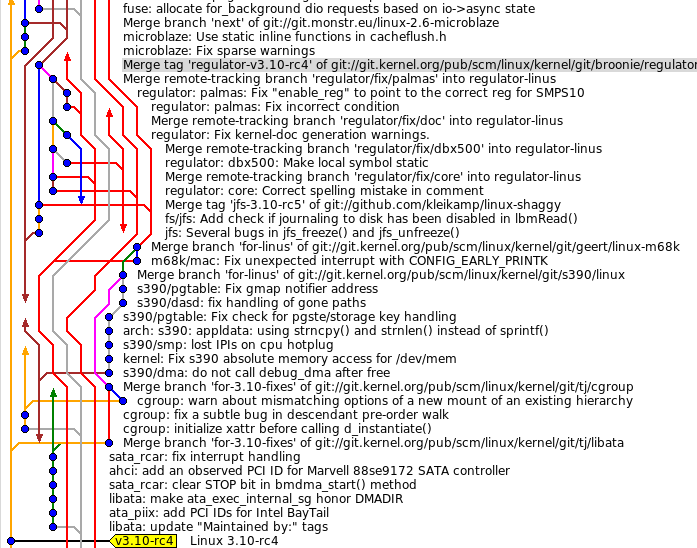
\includegraphics[width=0.47\textwidth]{figures/042dd_DAG.png}
	\caption{Merge Dag View}
	\label{fig:dag_view}
\end{figure}

\begin{figure}[h]
	\centering
	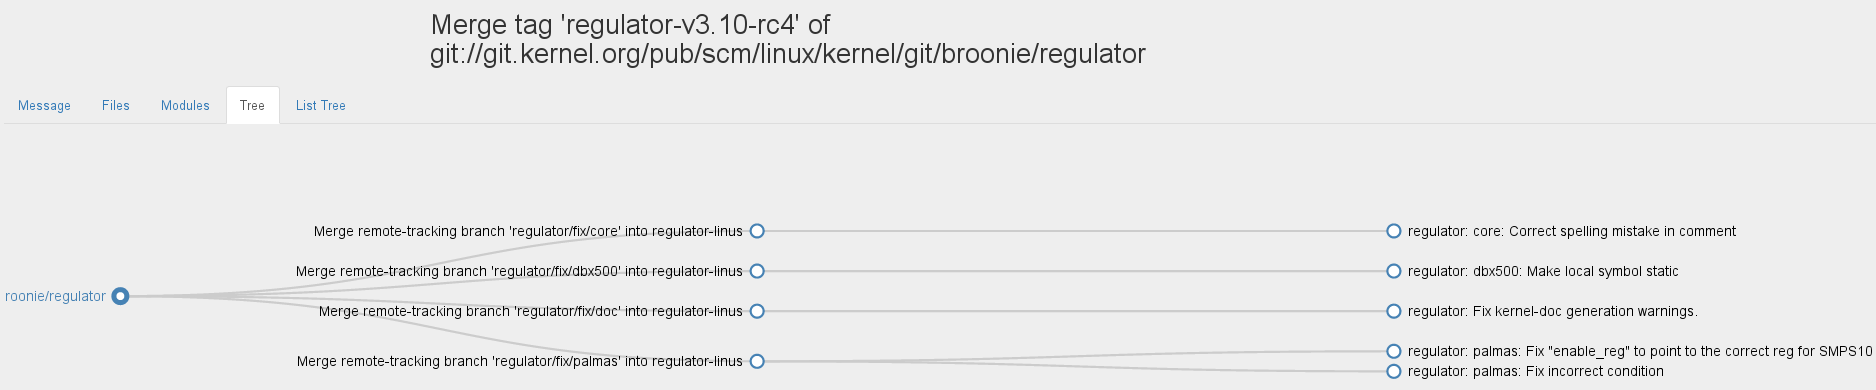
\includegraphics[width=0.47\textwidth]{figures/042dd_tree.png}
	\caption{Merge Tree View}
	\label{fig:tree_view}
\end{figure}

Our goal was to build a tool to enable maintainers to effectively navigate and
pull explanation of the changes performed to the kernel over a release.
Achieving this goal includes removing information that does not pertain to given
users. In figure \ref{fig:dag_view} and figure \ref{fig:tree_view}, we can
visually compare the results returned from gitk and our tool for the top-level
merge ``042dd60ca6dec9a02cefa8edd67de386e35755d6'' from kernel version 3.10.
The relevant information in both of these figures is identical, but the
presentation durastically changes our understanding of what we are seeing.

This merge is relatively small, containing only four merges, three of which
only contain a single commit, and the last containing two commits. With our
tool, we are able to immediately see what commits and merges pertain to our
section of the kernel. The DAG view of this provides almost no explanation,
futhermore, users must work to determine where this merge ends and the next one
begins.

Our tool further enhances our understanding by immediately giving us the files
that were edited and the modules. We are able to determine that three files,
``palamas-regulator.c'' had two lines added and two lines removed,
``dbx500-prcmu.c'' had 12 lines added and 12 lines removed, and ``core.c'' had
5 lines added and 2 lines removed in the merge. Finally, we are able to
determine that only the module ``regulator'' was modified in this merge, and
there were 5 commits in the merge to this module.


\subsection{Performance Evaluation}

Re-structuring the kernel into a tree changes the runtime for the structures.
Originally, we were performing all of our tree-navigation using recursive SQL
queries. Recursive queries have terrible performance, with the average response
time from the database being around 3 seconds for a single operation. We found
that it was far more time-efficient to load an entire tree directly into
memory, then iterate over the objects returned to build the tree structures,
than it was to have the dbms perform the tree traversals, building the specific
trees for a commit. At this time, we have re-implemented the breadcrumbs, the
files, and the main tree to enhance the response times. We will discuss some We
will discuss the changes made.

The breadcrumbs are generated at response
time, so they must be generated quickly. We began with a single recursive SQL
query, but was unable get the results in the required time, causing all result
pages to render slowly. We replaced the recursive query with a single query
that would grab the entire merge tree, rooted at the top-level merge.

The items returned from the database contained the commit id, the commit id of
the merge with the Linux kernel, and the next merge in the path to the
top-level merge.

We placed each item in the results into a dictionary using the commit id as the
key. Using the following method, we build the dictionary into a list of commit
IDs for the breadcrumbs.

\begin{verbatim}
current = cid
breadcrumbs = [cid]
while current is not top-level merge:
        breadcrumbs.append(current.next)
	current = current.next
return reverse(breacrumbs)
\end{verbatim}

This maintains the O(n) runtime for generating the breadcrumbs, while using an
iterative method for traversing the tree.

We use similar methods to generate the file information and the tree. Both are
generated asynchronously, allowing us to use spinners to help improve the user
experience. We are using AJAX requests to generate the asynchronous requests,
are are having very good results.

\subsection{Extendability}
Due to how the asynchronous requests are performed, it is possible to query the
server for the tree and file information directly, allowing other users to
build their own front-ends for working with our tree-based system.

The tree and file information is accessible through
http://li.turingmachine.org/data/tree/JSON/<commit id> and
http://li.turingmachine.org/data/files/JSON/<commit id>, respectively.
The tree is generated as many nested javascript objects. The tree response does
not contain any notion of the current commit and will only return the entire
merge tree.

The tree responses are generated as a single object. This object is the root
node of the tree, and may contain many objects with the same fields in the
``children'' field. The full response format for the tree looks like:

\begin{itemize}
        \item ``cid'': string, commit id
        \item ``name'': string, One-line log preview
        \item ``author'': string, Author's name
        \item ``mlinus'': string, commit id of top-level merge
        \item ``mnext'': string, commit id of the next merge on path to
                top-level
        \item ``children'': list, list of items with the same fields. Null if
                no children
\end{itemize}

The file responses contain only the files that the current merge or commit
works with. The response is a single object in the form of a tree. This object
is the root of the tree, and represents the current merge or commit. If the
current position in the tree is an inner node, the response will contain the
children in the ``children'' field, otherwise ``children'' will be null. The
full response format for the file response looks like:

\begin{itemize}
        \item ``cid'': string, commit id
        \item ``files'': list, list of tulples in the format
                \begin{enumerate}
                        \item Filename: string
                        \item Lines added: unsigned integer
                        \item Lines removed: unsigned integer
                \end{enumerate}
        \item ``mnext'': string, the commit id of the next merge toward the
                top-level merge
        \item ``children'': list, List of all child objects with the same
                fields. Null if no children.
\end{itemize}

\section{Future Work}
This project was implemented over the course of 4 months, interleaved with
other course projects and assignments. There are still many areas that could
use improvements before the full potential of our model can be reached and
understood with our tool. Here, we outline various areas that still need more
attention.

\subsection{Files}
We have limited functionality surrounding files, for both search and presented
information.

There is currently no functionality surrounding searching by filename. Use-case
2 may know what file they are editing and try to determine how it may work with
the other commits and merges in the module. It is possible that a third
use-case may arise, where the user wants to determine all commits that effect a
given file. In both cases, a bottom-to-top approach is used. With this
functionality, implementing the top-to-bottom search feature becomes trivial.

There is limited functionality to the presentation of the file information. At
a minimum, the patches for the commits can be displayed. The patches can then
be used for many more additional features. The patches can be used to piece
together parts of the file to generate a full patch at a given merge rather
than displaying each patch individually. The patches can also be used for
determining what kinds of changes were made, if the lines are being added,
removed, or replaced.

\subsection{Testing}
At this time, we have no evidence that our tool is able to improve the
work-flow of maintainers. We believe that the tool is able to improve the
work-flow and performance of maintainers because it is able to better assist
users because it provides cleaner mechanisms of working with the data. It is
able to provide more relevant information, while removing information that is
irrelevant to a given module or set of merges.

We could perform user-testing, or have some example cases where the tool is
used and the users provide feedback on how it improves or hurts their work
flow.

\subsection{Performance}
The modules and list tree view still use the old method of gathering the
information for the respective view type. For single commits or very small
merges, getting everything directly from the database and performing everything
server-side performs better than using the asynchronous requests, as there
isn't the overhead of multiple round trips; however, as the size of the merges
grow, the performance becomes far worse than the asynchronous system and in
some cases will time out. The asynchronous approach adds some overhead,
profiled at roughly 500ms, regardless of the response size. The asynchronous
approach has many benefits, over building the response on the server, including
the ability to add spinners, which is an improvement to user-experience over
looking at a blank page. Further work can be done to improve the results beyond
the response time of 500ms using improved queries and more efficient methods of
building the tree.

\section{Conclusion}

\evantodo{DO IT! JUST DO IT!}

\bibliographystyle{plain}
\bibliography{citations}

% \balance
\end{document}
